\documentclass[../main/report.tex]{subfiles}
\begin{document}
\section{Testing of Communication Channels}
Prototyping and testing of communication channels were essential in making our system function properly.
We needed to get comfortable with the MCU programming environment, learn how configure the MCU properly, learn about bus protocols etc.
Our project PCB was delivered to us only two weeks prior to project deadline, and therefore we needed to create a working prototype of these aspects before our actual system was ready to use.

Our prototype setup is shown in concept and in actuality in Figure \ref{prototype}.
We tested bus communication with EBI between MCU and FPGA, video output signals with HDMI from FPGA, controlling it with a debugger connected to the MCU.
Note that we used a DVI cable instead of a HDMI cable to connect to the GPIO pins as that was more readily available to us. The two protocols are conventiently pin-compatible and interchangeable.

\begin{figure}[htp]
\centering
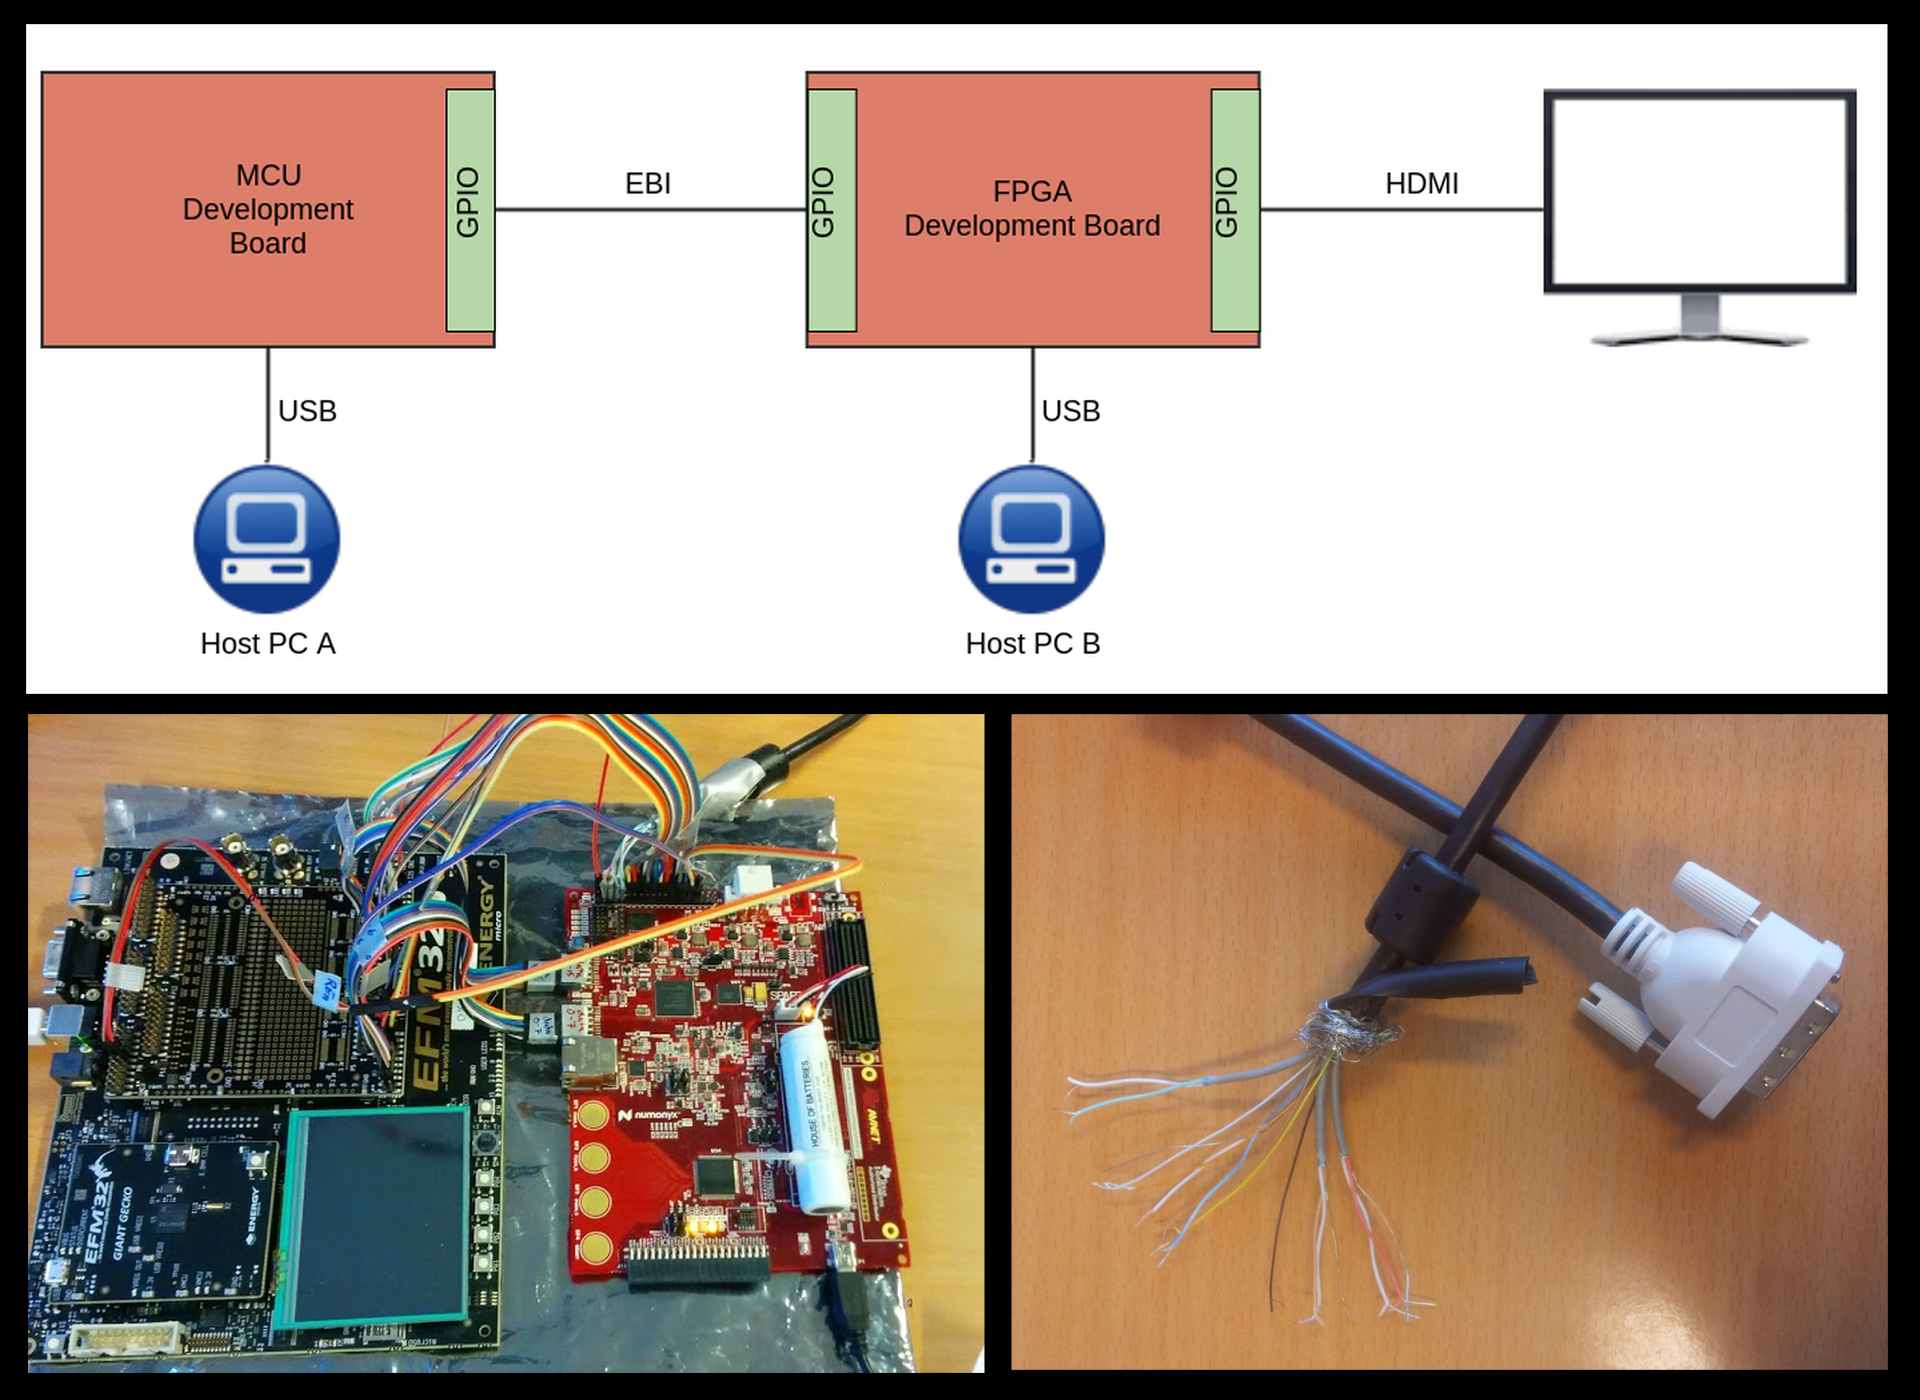
\includegraphics[width=\textwidth]{../diagrams/prototype_complete.png}
\caption{Prototype of Communication Channels}
\label{prototype}
\end{figure}

\subsection{EBI Test}
\todo{Rewrite paragraphs to more test-like format}
For our first test, we created a working EBI communication between MCU and FPGA.
Creation of the MCU program was aided by publicly available Silicon Labs examples and documentation.
Filtering away the complicated setup of the MCU development board itself, none of which we need for our final system, was difficult.
But the stripped-down EBI code we were left with in the end was relatively short and easy to understand.
We strived to use the exact same GPIO pins on the prototype as the ones we have routed in our PCB.

For the FPGA side of the bus we used the exercise framework of TDT4255 Computer Architecture as a starting point.
It is a VHDL project that has some memory and a module for programming the FPGA and reading its memory.
Fortunately, the EBI protocol is simple enough to let us wire the MCU's address lines, data lines, and write enable signal directly to the FPGA memory module's corresponding ports.
This worked because the memory module ran at a higher clock frequency than the MCU, and therefore had at least one rising clock edge every time the MCU asserted write enable.

To get an understanding of the data rate on the bus, we analyzed the writes with a logic analyzer.
The measured write frequency was about 1.5 MHz.
Reading the specifications for the MCU clock, we found that we could change the clock band from a 14 MHz frequency band to 28 MHz.
A new measurement of the bus showed an improved write frequency of 3.2 MHz.

\begin{figure}[htp]
\centering
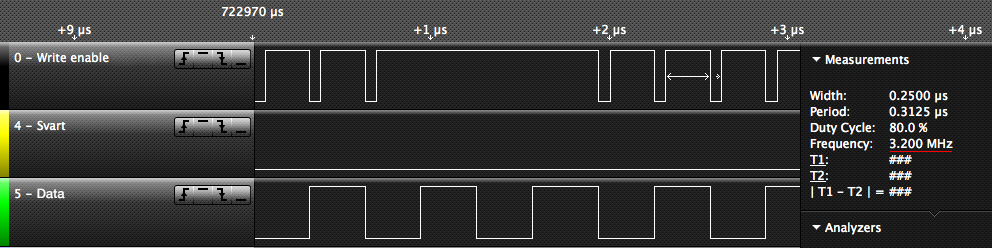
\includegraphics[width=\textwidth]{../diagrams/ebi_bus_write_speed.png}
\caption{The frequency of writes, as measured with a logic analyzer}
\label{ebi_bis_write_speed}
\end{figure}

\subsection{HDMI Test}
\todo{Describe this test}

\subsection{EBI \& HDMI Test}

\begin{wrapfigure}{r}{0.3\textwidth}
\centering
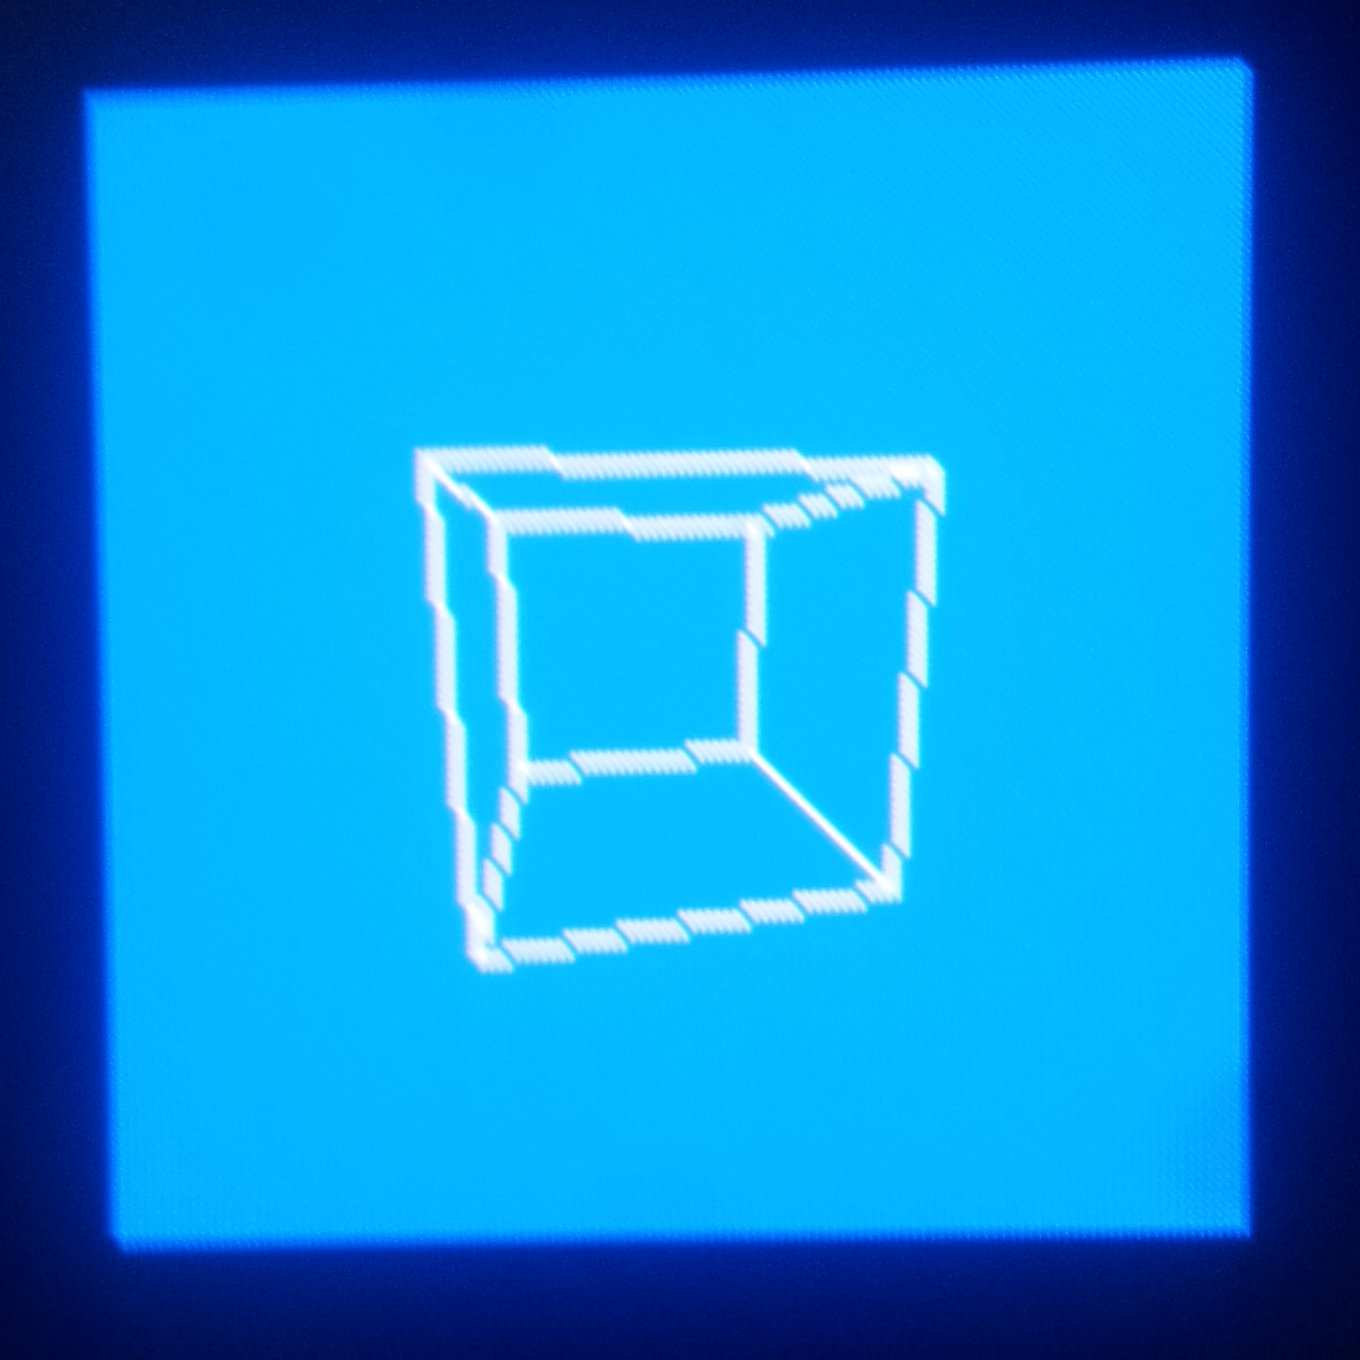
\includegraphics[width=0.3\textwidth]{../diagrams/prototype_demo.png}
\caption{Screenshot of test demo}
\label{prototype_demo}
\end{wrapfigure}

For a combined prototype we connected these two communication channels in a system that let the MCU write pixel values to screen through the FPGA.
A short program on the MCU ran a simple "demo" of a spinning cube in a 128 by 128 pixel frame on screen.
Note that at this point in time, the GPU architecture was not yet completed.
As such, our prototype was not one for the whole project system, but merely for our two main communication channels.
SRAM chips and their interface were also not part of this prototype.
Communication to external SRAM chips was not tested prior to receiving our PCB.
Instead, we used two memory modules internally on the FPGA for two small framebuffers.

With this test, we made sure that we could send HDMI output from a memory framebuffer, and even switch between two buffers. 
\todo{Explain more detailed what this means}

We played with the clock speed of both MCU and FPGA on this test.
Framebuffer for our HDMI output was switched as soon as the MCU finished writing its next frame, making the frequency of frame updates directly dependent on the speed of transfers over our EBI bus.
The consequence was a visual feedback gave us an imprecise but useful indication of the speed of our EBI transfers.
As we expected, if the MCU clock speed was higher than the FPGA clock speed, we would get "artifacts" on screen.
That is, not every transfer would be received on the FPGA side, leaving "old" pixel values in our framebuffers.

\end{document}